\documentclass[twoside, openright, 12pt]{book}
\sloppy

% Preamble
% General Setup
\usepackage{ifthen}		% If-Then-Statements
\usepackage{pdfpages}
\usepackage{hyperref}		% Hyperlinks & PDF specific information
\hypersetup{
	pdftitle={Master thesis - Philipp Schwetschenau},
	pdfsubject={Master thesis},
	pdfauthor={Philipp Schwetschenau},
	pdfborder={0 0 0}
}
\usepackage[nounderscore]{syntax}

% Language & Encoding
\usepackage[T1]{fontenc}
\usepackage[USenglish]{babel}
\usepackage[fixlanguage]{babelbib}
\usepackage[utf8]{inputenc}
\usepackage{blindtext}
\usepackage{caption}

% Page Geometry
\usepackage[a4paper]{geometry}
\geometry{
	twoside,
	top=3cm,
	bottom=3cm
}

% Literature
\usepackage{url}
\usepackage[sort&compress,square,comma,authoryear]{natbib}

% Fonts & Symbols
\usepackage{latexsym}		% Rare symbols
\usepackage{amsfonts}		% Math fonts
\usepackage{amssymb}		% Symbols
\usepackage{amsmath}		% Symbols
\usepackage{lmodern}		% "Latin Modern" ("Computer Modern"++)

\newcommand{\origttfamily}{}	% Separator for typewriter
\let\origttfamily=\ttfamily
\renewcommand{\ttfamily}{\origttfamily \hyphenchar\font=`\-}


%
% Document Layout

\usepackage[activate]{pdfcprot}	% margin kerning

% Header & Footer
\usepackage{fancyhdr}		% format headers
\pagestyle{fancy}
\fancyhf{}
\setlength{\headheight}{15pt}
\fancyhead[LE,RO]{\sffamily \thepage}
\fancyhead[RE]{\sffamily \nouppercase{\leftmark}}
\fancyhead[LO]{\sffamily \nouppercase{\rightmark}}
\renewcommand{\headrulewidth}{0.4pt}
\fancypagestyle{plain}{
	\fancyhead[RE,LO]{}
	\renewcommand{\headrulewidth}{0pt}
}
\fancypagestyle{simple}{
	\fancyhead[RE,LO]{}
	\renewcommand{\headrulewidth}{0pt}
}
\fancypagestyle{light}{
	\fancyhead[RE,LO]{}
}

% ClearDoublePage fix
\makeatletter 
\def\cleardoublepage{\clearpage\if@twoside \ifodd\c@page\else% 
\hbox{}% 
\thispagestyle{simple}
\newpage% 
\if@twocolumn\hbox{}\newpage\fi\fi\fi}
\makeatother 

% Headlines
\usepackage{titlesec}
\setcounter{secnumdepth}{3}
\titleformat{\chapter}[display]%
	{\huge\center\bf}%
	{\large\mdseries CHAPTER \thechapter}%
	{0cm}{}[\vspace{2ex}\titlerule]
\titlespacing*{\chapter}{0pt}{0ex}{8ex}
\titleformat{\subsubsection}{\normalsize\bfseries}{\thesubsubsection}{.75em}{}
\titleformat{\paragraph}[runin]{\bfseries}{}{0pt}{}[.]
\titleformat{\subparagraph}[runin]{\itshape}{}{0pt}{}[.]

% Table of Contents
\usepackage[titles]{tocloft}

\setlength{\cftbeforetoctitleskip}{0ex}
\setlength{\cftaftertoctitleskip}{0ex}
\renewcommand{\cfttoctitlefont}{}

\setlength{\cftbeforeloftitleskip}{4ex}
\setlength{\cftafterloftitleskip}{1ex}
\renewcommand{\cftloftitlefont}{\LARGE}

\setlength{\cftbeforelottitleskip}{4ex}
\setlength{\cftafterlottitleskip}{1ex}
\renewcommand{\cftlottitlefont}{\LARGE}

\newcommand\listingname{Verzeichnis der Listings}
\newlistof[chapter]{listing}{lst}{\listingname}
\setlength{\cftbeforelsttitleskip}{4ex}
\setlength{\cftafterlsttitleskip}{1ex}
\renewcommand{\cftlsttitlefont}{\LARGE}

\newcommand\theoremsname{Theoremverzeichnis}
\newlistof[chapter]{theorems}{lthm}{\theoremsname}
\setlength{\cftbeforelthmtitleskip}{4ex}
\setlength{\cftafterlthmtitleskip}{1ex}
\renewcommand{\cftlthmtitlefont}{\LARGE}

\setcounter{tocdepth}{2}
\setlength{\cftbeforechapskip}{1.0ex}
\setlength{\cftbeforesecskip}{0ex}
\setlength{\cftbeforesubsecskip}{-.2ex}
\newcommand\tocentry[1]{\addcontentsline{toc}{chapter}{#1}}
\newcommand{\ttsubsection}[1]{\subsection[\texorpdfstring{\texttt{\slshape #1}}{#1}]{\texttt{#1}}}
\newcommand\addtotheorems[2]{
	\refstepcounter{theorems}
	\addcontentsline{lthm}{theorems}{\protect\numberline{\thetheorems}\textbf{#1:} #2}
}
\newcommand\addlistspace[1]{
	\addtocontents{#1}{\vspace{1.3ex}}
}

% Glossar
\usepackage[number=none,style=altlist]{glossary}
\renewcommand{\glosslabel}[2]{\sffamily #2}
\makeglossary


%
% Page Elements

% Captions & Figures
\usepackage{graphicx}		% include graphics
\graphicspath{{./figures/}}

% Tables
\usepackage{booktabs}

% Theorems
\usepackage{framed}		% Frames for theorems.
\usepackage[framed,thmmarks,amsmath]{ntheorem}	% extended theorem enviroments
\usepackage{shadethm}		% theorems with colored background
\theoremheaderfont{\sffamily\bfseries}
\theorembodyfont{}
\theoremstyle{break}
\theoremseparator{.}
\theoremindent0cm
\theoremsymbol{}

\newshadetheorem{xtheorem}{Theorem}[chapter]
\newshadetheorem{xlemma}[xtheorem]{Lemma}
\newshadetheorem{xdefinition}[xtheorem]{Definition}
\newshadetheorem{xrequirement}[xtheorem]{Requirement}

\newenvironment{theorem}[1][]{%
	\addtotheorems{Theorem}{#1}
	\begin{xtheorem}[#1]%
}{\end{xtheorem}}
\newenvironment{lemma}[1][]{%
	\addtotheorems{Lemma}{#1}
	\begin{xlemma}[#1]%
}{\end{xlemma}}
\newenvironment{definition}[1][]{%
	\addtotheorems{Definition}{#1}
	\begin{xdefinition}[#1]%
}{\end{xdefinition}}
\newenvironment{requirement}[1][]{%
	\addtotheorems{Requirement}{#1}
	\begin{xrequirement}[#1]%
}{\end{xrequirement}}

\newshadetheorem{xapxtheorem}{Theorem}[section]
\newenvironment{apxtheorem}[1][]{%
	\addtotheorems{Theorem}{#1}
	\begin{xapxtheorem}[#1]%
}{\end{xapxtheorem}}

\theoremstyle{nonumberplain}
\theoremseparator{.}
\theoremheaderfont{\sffamily\itshape}
\theoremsymbol{\ensuremath{\Box}}
\newtheorem{proof}{Proof}
\newtheorem{apxproof}{Proof}

% Listings
\usepackage{listings}
\lstset{
	basewidth={0.5em,0.45em},
	frame=lines,
	framerule=\lightrulewidth,
	captionpos=b,
	lineskip=-1pt,
%	float=hbt,
	xleftmargin=1cm,
	xrightmargin=1cm,
	aboveskip=0.5cm,
	belowskip=0.5cm,
}
\lstnewenvironment{java}[2]{
	\refstepcounter{listing}
	\addcontentsline{lst}{listing}{\protect\numberline{\thelisting}#1}
	\lstset{
		language=C++,
		basicstyle=\ttfamily,
		commentstyle=\sffamily,
		lineskip=-2pt,
		tabsize=4,
		#2
	}
}{}
\lstdefinelanguage{pseudocode}{
	sensitive=true,
	alsodigit={:},
	morekeywords={
		Algorithmus,Eingabe:,Ausgabe:,Variablen:,%
		when,if,then,else,end,atomic,out,%
		case,is,repeat,while,do,until},
}
\lstdefinelanguage[distributed]{pseudocode}
	[]{pseudocode}{
	alsodigit={:},
	morekeywords={Async,Sync,%
		Constants:,Variables:,Input:,Action:,Action,%
		send,to,from},
	deletekeywords={Algorithmus,Eingabe:,Ausgabe:,Variablen:}
}
\newcommand{\setpseudocode}[2]{
	\lstset{
		% Syntax
		language=[#1]{pseudocode},
		mathescape=true,
		escapechar=\#,
		tabsize=4,
%		gobble=4,
		literate={:=}{{$\gets$}{\:}}2 {->}{{$\rightarrow$}{\:}}2,
		% Style
		basicstyle=\rmfamily,
		commentstyle=\sffamily,
		moredelim=[is][\itshape]{//}{//},
		moredelim=[il][\sffamily]{**},
		% Layout & Placement
		numbers=left,
		numberstyle=\tiny,
		columns=flexible,
		breaklines=true,
		breakatwhitespace=true,
		breakindent=2em,
		% User defined
		#2
	}
}
\lstnewenvironment{distalg}[2]{%
	\refstepcounter{listing}
	\addcontentsline{lst}{listing}{\protect\numberline{\thelisting}#1}
	\setpseudocode{distributed}{#2}
}{}
\lstnewenvironment{pseudocode}[2]{%
	\refstepcounter{listing}
	\addcontentsline{lst}{listing}{\protect\numberline{\thelisting}#1}
	\setpseudocode{}{#2}
}{}

\newcommand\textcall[1]{\textsc{#1}}
\newcommand\call[2]{\ensuremath{\operatorname{\textcall{#1}}(#2)}}
\newcommand\callname[2]{\ensuremath{\operatorname{#1}(#2)}}
\newcommand\topin[1]{\ensuremath{\operatorname{In}({#1})}}
\newcommand\topout[1]{\ensuremath{\operatorname{Out}({#1})}}


%
% Inline
\usepackage{url}		% Cite URLs
\usepackage{numprint}		% Format numbers
\newcommand\notice[1]{}		% Notice
\newcommand\seppar{ \vspace{2ex} \noindent } % New paragraph
\newcommand\name[1]{{\em #1}} 	% Names


\newenvironment{BNF}
  {\captionsetup{type=lstlisting}}
  {}

\begin{document}

%
% Titelseite
\begin{titlepage}
\newlength{\detailwidth}
\newlength{\detaildescriptionwidth}
\settowidth{\detailwidth}{Eingereicht:~~ Prof. Dr.-Ing. habil. Winfried E. Kühnhauser}
\settowidth{\detaildescriptionwidth}{Studies:~~} 
\begin{center}

\vfill {
	
\includegraphics[width=6cm]{logo-tu-ilmenau.jpg}
	\vspace{8ex}
}

\begin{normalsize}Technische Universität Ilmenau \\
Fakultät für Informatik und Automatisierung \\
Institut für Praktische Informatik und Medieninformatik \\
Fachgebiet für Verteilte Systeme und Betriebssysteme        
\end{normalsize}


\vfill {\large
	Masters thesis\\ \vspace{2ex}
	\LARGE \textbf{Graphical Specification Language for the Entity-Labeling Aspect} \\ \vspace{2.5ex} 
	\normalsize Submitted by: \\
	\Large Philipp Schwetschenau \\ \vspace{3ex} 
}
\vfill \parbox{\detailwidth}{
	\makebox[\detaildescriptionwidth][r]{Supervisor:~~} Prof. Dr.-Ing. habil. Winfried E. Kühnhauser \\
	\makebox[\detaildescriptionwidth][r]{Supervisor:~~} Peter Amthor \\
	\vspace{2ex} \\
	\makebox[\detaildescriptionwidth][r]{Studies:~~} Computer science\\  
	\makebox[\detaildescriptionwidth][r]{Matriculation no.:~~} 46756  
	\vspace{2ex} \\
	\makebox[\detaildescriptionwidth][r]{Submission date:~~} Ilmenau, 29. November 2018 
}
\vspace*{\fill}
\end{center}
\end{titlepage}

\mbox{}
\thispagestyle{empty}
\cleardoublepage

% Gliederung
\pagenumbering{roman}
\setcounter{page}{1}
\tableofcontents

% Abbildungsverzeichnis
\cleardoublepage
\listoffigures
\tocentry{List of figures}

%\listoflisting
%\tocentry{\listingname}

%
% Citing

% Author 1 et al. [1234]
%\cite{Harrison75a}

% Author 1, Author 2, Author 3 [1234]
%\cite*{Harrison75a}

% [Author 1 et al. 1234]
%\citep{Harrison75a}

% [Author 1, Author 2, Author 3 1234]
%\citep*{Harrison75a}



% Inhalts-Teil
\cleardoublepage
\pagenumbering{arabic}
\chapter{Introduction}
\label{introduction}

\section{Domain} 
\label{domain}
With the increasing number of IT systems, securing these systems became an obvious and important issue.
For this purpose many security models and model families were developed for a wide field of application domains over the last years.

Formal security models offer possibilities to analyze them concerning security properties.
However, because quantity and variety of these models grow just as much as their relevance for security-critical applications the model-based security engineering process became more complex and therefore error-prone to human deviations.

\citet*{Amthor18} proposed a new approach called Aspect-oriented Security Engineering (AOSE) which claims to close semantic gaps between steps in the security engineering process (requirements, informal policy, formal model) to reduce the potential impact of human errors.
This approach roughly adopts the idea of the aspect-oriented programming paradigm.
It tailors all steps to aspects, which are non-functional requirements of the engineering process like determining requirements of policy semantics or analyzing certain security goals.
There are two major classes for aspects regarding AOSE: related to policy semantics and to policy analysis.

One possible aspect of the former is the Entity Labeling Aspect (EL).
It is designed to formally specify policy semantics typically found in operating systems and middleware systems.
Therefore it bridges the gap and supports the transformation between informal policy and formal model.
EL classifies model components into six semantic categories.
The notation is on a mathematical basis and uses concepts like sets, assignments or constraints.



\section{Motivation} 
\label{motivation}
The goal of reducing the impact of human errors by closing semantic gaps as much as possible with the help of AOSE/EL requires handling another formal notation, which is, in this case, EL itself and its classification into the six semantic categories.
To support working with this approach, especially for the communication between different groups of people involved like model engineers, security architects, software developers or future administrators, who have to cooperate and coordinate and all have different levels of experience, \citet*{Amthor18} considers a graphical representation to be helpful to enhance the transition between informal and formalized notation.

\citet*{Amthor18} already uses visual representations to illustrate examples.
However, the representations are not described in detail as well as they are inconsistent and ambiguous regarding several parts of the formalization (e.g.\ arrows can have several meanings and there is no way to specify functions with multiple input parameters).
So these visualizations are appropriate to underline and support the engineering of an already formalized policy after EL-based model engineering, but are not suitable for independent modeling on a stand-alone level, because they are not equivalent to their formalized mathematical counterpart.

There are two types of visualization \cite{Amthor18} uses, which have different levels of abstraction: 
One is based on the actual model components and visualizes them and their relationships.
The other one is based on a higher level of abstraction and visualizes the EL with its structure of semantic categories and their relationships.

There are other visual notations like UML or ERD, which have in common that they are tailored to particular needs in special application domains, so they can not be applied here, but may give inspiration on how to model certain semantics and relationships.

Eventually to be able to independently and visually model and work on EL-based policies there is need for an unambiguous formal graphical specification language.



\section{Goal}
\label{goal}
The main goal is to develop a graphical specification language for EL-based security polices.
This should focus on clean and unambiguous semantics of the language.

The use of the language should be as simple as possible and as comprehensive as needed.
Therefore its appearance and elements should be clear and well-structured.
A selection of appropriate symbols and geometrical shapes for their equivalent model counterparts has to be made regarding an intuitive understanding and workflow.
This selection should not be designed contradictory or conflicting to already established notations, especially those, which may be used in the context of security engineering.

It should be evaluated how feasible and reasonable it is to develop equivalent counterparts for every possible element and relationship in context of EL and to display all of them at once.
This may also lead to the question how the visualization is related to a visualization on a higher abstraction level and how they are connected and might be managed.
The latter may be investigated as an optional goal.

In addition to that a GUI-based editor should be developed as a prototype to make use of the proposed graphical specification language.



\section{Structure}
\label{structure}




\cleardoublepage
\chapter{Fundamentals}
\label{fundamentals}
This chapter provides information to all fundamentals necessary for this thesis.
It will serve as basis for all design decisions in the following chapter~\ref{gsl_design} and chapter~\ref{editor_design}.

Section \ref{security_models} introduces the security models HRU and RBAC as well as the Security Model Core.
Section \ref{AOSEEL} focuses on the Aspect-oriented Security Engineering (AOSE) proposed by \citet*{Amthor18}.
It covers the Entity-Labeling Aspect in particular, one aspect of AOSE, which is going to be essential regarding the task to design a graphical specification language for it in chapter~\ref{gsl_design}.
In section~\ref{graphical_notations} the well-established graphical notations UML and ER are described.
Based on human optical perception and gestalt laws section~\ref{gestalt_laws_and_human_optical_perception} provides information on how we perceive and evaluate visual impressions regarding two-dimensional forms and structures.
In the last section~\ref{gui_design} information on how to design a software graphical user interface are given with respect to common best practices like design patterns and modern usability.

\section{Security models}
\label{security_models}
Security policies are sets of rules to fulfill security related requirements of a system.
To actually be able to work with such policies and also in context of analyzing them, they have to be formalized as an instance of a security model.
In context of model-based security engineering these security models are obviously the most important artifact.
So this section introduces the HRU security model as well as the family of RBAC models with its concepts and elements.
Furthermore this section will present a concept to express all types of security models in form of a single model, the Security Model Core.

\subsection{HRU}
\label{HRU}
The HRU security model \citep*{Harrison75a} is a fundamental, dynamic access control model.
It manages permissions of subjects on objects with the help of an state automaton and access control matrices.
While subjects are active (e.g. users), objects are passive (e.g. files).

\begin{xdefinition}[HRU] 
A HRU model is a deterministic automaton
$(Q, \Sigma , \delta , q_{0})$ with 
$Q = 2^S \times 2^O \times M$ as state space, 
$M = \lbrace m|m:S \times O \rightarrow 2^R \rbrace$ as set of access control matrices, 
$\Sigma$ as input alphabet, 
$\delta : Q \times \Sigma \rightarrow Q$ as state transition function and 
$q_0 \in Q$ as initial state.
\end{xdefinition}



\subsection{RBAC}
\label{RBAC}
Due to its usage of access control matrices the HRU model does not scale well with an increasing number of subjects and objects.
The family of role-based access control models (RBAC) counter this more effectively by using one stage of indirection.
For this RBAC models introduce the concept of roles \citep{Sandhu96}.
On the one hand every user is mapped to a set of roles.
On the other hand every role is mapped to a set of permissions.

\begin{xdefinition}[RBAC] 
A RBAC$_0$ model is a tuple $(U, R, P, S, UA, PA, user, roles)$ with 
$U$ as set of \textit{users}, 
$R$ as set of \textit{roles}, 
$P = 2^{O \times OP}$ as set of \textit{permissions} 
($O$ is the set of \textit{objects} and 
$OP$ the set of \textit{operations}), 
$S$ as set of \textit{sessions}, 
$UA \subseteq U \times R$ as \textit{user-role relation}, 
$PA \subseteq P \times R$ as \textit{permission-role relation}, 
$user: S \rightarrow U$ as assignment, that maps every session to a user and
$roles: S \rightarrow 2^R$ as assignment, that maps every session to set of roles.
\end{xdefinition}

RBAC is called family of security models, because there is a base model (RBAC$_0$) and advanced models that extend the base model.
RBAC$_1$ extends RBAC$_0$ with a role hierarchy, because in reality it turned out that roles are often combinations of other already existing roles.
This reduces redundancy and improves its scaling behavior with increasing number of users and objects even further.
RBAC$_2$ extends RBAC$_0$ with a constraints component $C$ to restrict values for certain model components.
RBAC$_3$ combines RBAC$_1$ and RBAC$_2$.

In contrast to HRU RBAC is static.
Due to not being dynamic a RBAC model can always just reflect a snapshot in time.
To make it dynamic there is a model called DRBAC, which combines the RBAC$_3$ model with the deterministic state automaton of the HRU model.

\begin{xdefinition}[DRBAC] 
A DRBAC model is a tuple 
$(Q, \Sigma , \delta , q_{0}, OP, R, RH, C)$ with
$Q = 2^U \times 2^O \times 2^P \times 2^S \times 2^{\mathit{PA}} \times 2^{\mathit{UA}} \times \mathit{USER} \times \mathit{ROLES}$ as state space, where $U, O, P, S, PA, UA, RH, C$ is defined just as in the RBAC$_3$ model, 
$\mathit{USER} = \lbrace user|user: S \rightarrow U \rbrace$ as set of mappings that maps sessions to users, 
$\mathit{ROLES} = \lbrace roles|roles: S \rightarrow 2^R \rbrace$ as set of mappings that maps sessions to roles, 
$\Sigma = OP \times X$ as input alphabet, 
$\delta : Q \times \Sigma \rightarrow Q$ as state transition function, 
$q_0 \in Q$ as initial state and 
$OP, R, RH, C$ as static component.
\end{xdefinition}



\subsection{Security Model Core}
\label{model_core}
Over the years many different security models emerged for special purposes and requirements.
They heavily vary and differ in their structure and design.
Comparing them or even parts of them for analysis or evaluation purposes is not always possible per se.
Methods to analyze a model concerning a given security property have to be adapted to every model they should run on.
So \cite{Poelck14} proposed the Security Model Core to describe and formalize all possible security models in one meta model in a homogeneous way.

\begin{xdefinition}[Security Model Core]
\label{def:SecurityModelCore}
The Security Model Core is a 5-tuple 
$(Q, \Sigma , \delta , q_{0}, E)$ with 
$Q$ as state space,
$\Sigma$ as input alphabet, 
$\delta: Q \times \Sigma \rightarrow Q$ as state transition function, 
$q_0$ as initial state and 
$E$ as static extension vector.
\end{xdefinition}

The definition of model components depends on the specialization of the corresponding model core and is done in six steps by identifying and defining those components.



\section{Aspect-oriented Security Engineering and Entity-Labeling Aspect}
\label{AOSEEL}


\subsection{Aspect-oriented Security Engineering}
\label{AOSE}


\subsection{Entity-Labeling Aspect}
\label{EL}




\section{Graphical notation models}
\label{graphical_notations}

\subsection{Unified Modeling Language}
\label{UML}
The \textit{Unified Modeling Language} (UML) is a graphical modeling language to specify, visualize, design and document software \citep{UML}.
The current version of UML (2.5) contains 14 different types of diagrams.
Every diagram illustrates according to one specific aspect.
UML diagrams are classified into static and dynamic types, but they can have fuzzy borders and mixed forms as well.
Static diagram types describe structural properties, dynamic diagram types behavioral properties.

Components an UML diagram is build up with are classified into \textit{elements}, \textit{relationships}:

\begin{description}
\item[1) Elements]\hfill \\
Elements are the main objects in a UML diagram.
Graphically elements are based on closed shapes like boxes or ellipses.
They usually have a name or identifier in form of text in the center of their shape. Horizontal lines can be used to separate an element into two or more sections (see \textit{class diagram}). \\
Examples: Classes, components, nodes, objects, packages (see figure \ref{fig:UML_elements})

\begin{figure}[htb]
	\centering
	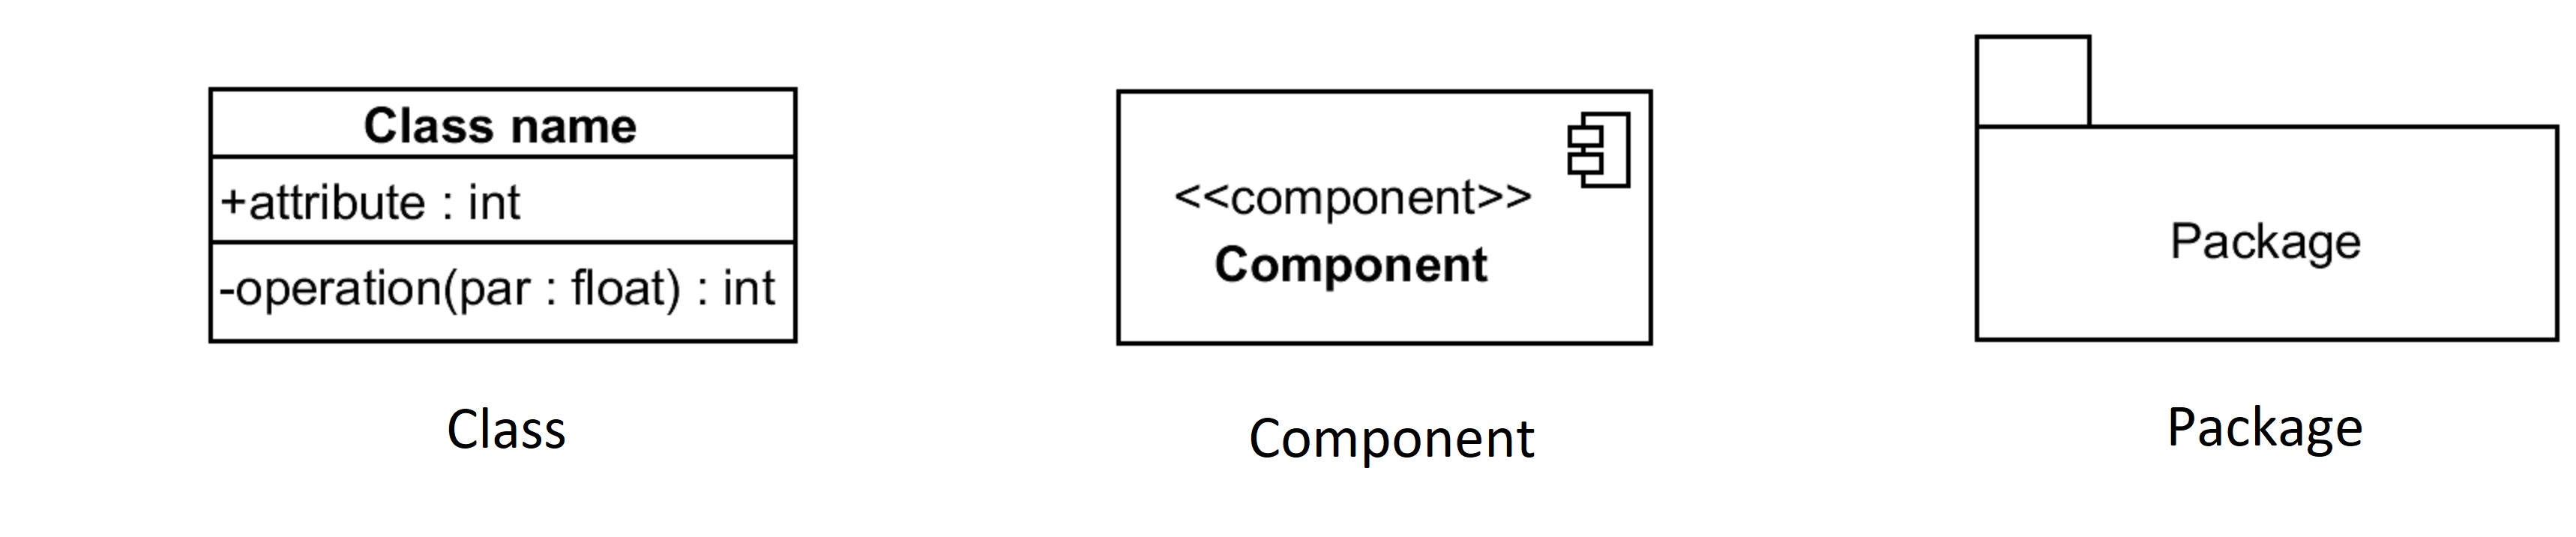
\includegraphics[scale=0.6]{../figures/chapter2/UML_elements.png}
	\caption{Selection of UML elements}
	\label{fig:UML_elements}
\end{figure}

\item[2) Relationships]\hfill \\
Relationships can connect two or more elements.
Graphically relationships are based on lines.
Optionally they can have a shape at one end to indicate some kind of direction.
They can vary in form by having differently drawn lines (solid, dotted), shaped arrows.
They can have several angles (preferable $90^{\circ}$ or $45^{\circ}$) to run on a clearly laid out path.
Lines do not collide if possible. \\
Examples: Dependency, association, generalization, include, extend (see figure \ref{fig:UML_relationships})

\begin{figure}[htb]
	\centering
	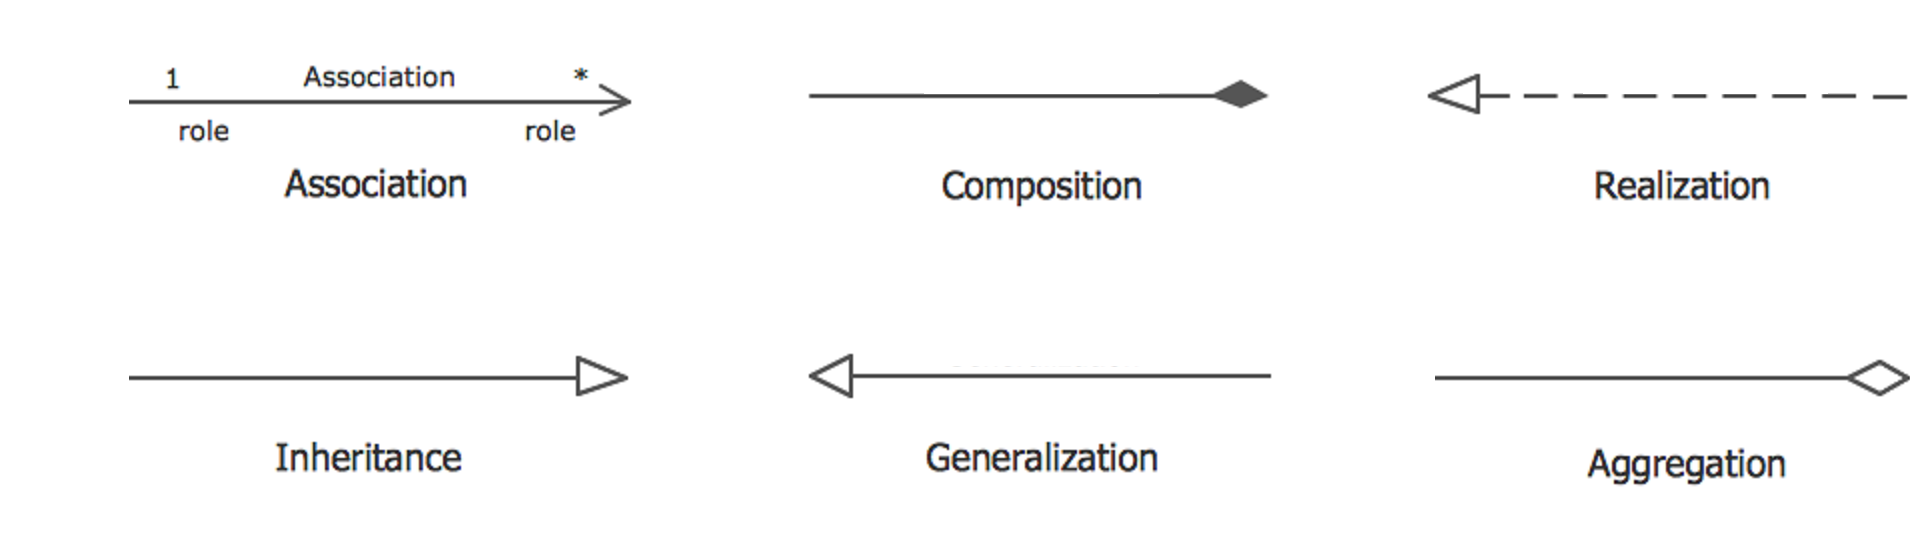
\includegraphics[scale=0.6]{../figures/chapter2/UML_relationships.png}
	\caption{Selection of UML relationships}
	\label{fig:UML_relationships}
\end{figure}
\end{description}

\noindent 
Class diagrams can have different levels of detail.
For example the class element has a simple symbolic form as well as an extended form with detailed information about its key words, attributes and operations (see figure \ref{fig:Class}).

\begin{figure}[htb]
	\centering
	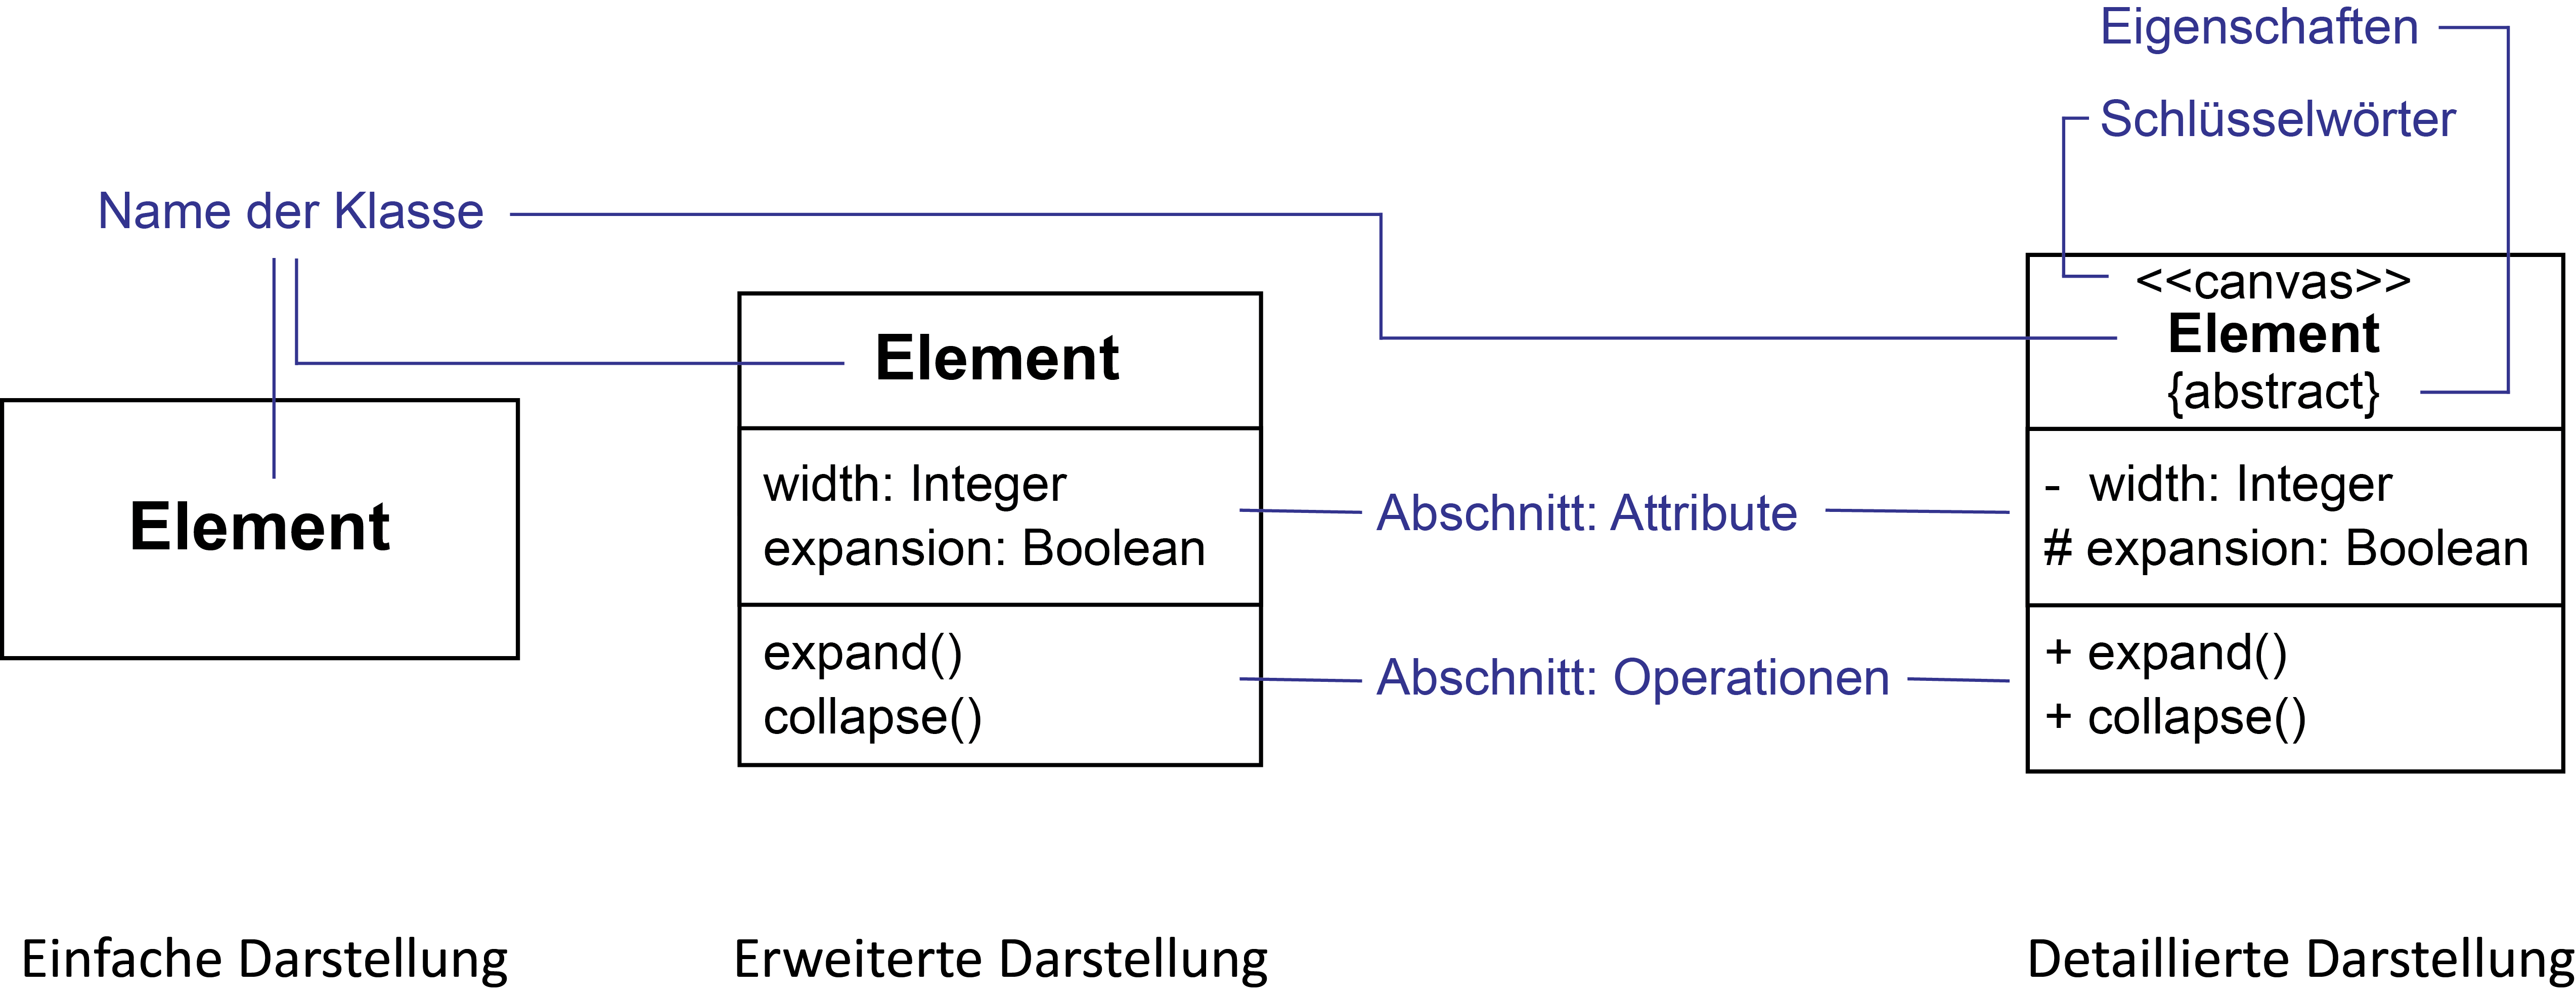
\includegraphics[scale=0.6]{../figures/chapter2/UML_Klassen2.png}
	\caption{Class diagrams with different level of detail}
	\label{fig:Class}
\end{figure}
 
\noindent 
UML has symbols and textual identifiers to visualize certain properties.
Class diagrams for example have the following symbols to indicate visibility or attributes and operations: + for \textit{public}, \# for \textit{protected} and - for \textit{private}.
With \textit{multiplicity} an element can be constrained regarding kind and number of its values.
The format for its bounds in BNF\footnote{Backus-Naur form} is defined by the UML specification 2.5 \citep{UML} as in listing \ref{BNF_multiplicity}.

\setlength{\grammarparsep}{10pt plus 1pt minus 1pt} % increase separation between rules
\setlength{\grammarindent}{13em} % increase separation between LHS/RHS 

\vspace{0.4cm}
\noindent
\begin{BNF}
\fbox{
\parbox[b]{\textwidth}{
\begin{grammar}
<multiplicity> ::= <multiplicity-range> [ [ `$\lbrace$' <order-designator> [ `,' <uniqueness-designator> ] `$\rbrace$' ] |
[ `$\lbrace$' <uniqueness-designator> [ `,' <order-designator> ] `$\rbrace$' ] ]

<multiplicity-range> ::= [ <lower> `..' ] <upper>

<lower> ::= <value-specification>

<upper> ::= <value-specification>

<order-designator> ::= `ordered' | `unordered'

<uniqueness-designator> ::= `unique' | `nonunique'
\end{grammar}
}
}
\caption{UML multiplicity syntax in BNF}
\label{BNF_multiplicity}
\end{BNF}
\vspace{0.3cm}

\noindent
For the sake of convenience we assume the literal <value-specification> being an integer number or * for infinite.

Furthermore it is worth mentioning that UML does not use any color for its diagrams.
This makes it compatible, easy and fast for hand-drawing.
Coloring always remains an not officially specified option to highlight certain parts of a diagram, e.g. to set a focus for an accompanying text.


\subsection{Entity-Relationship model}
\label{ER}
An entity-relationship model (ER model) is a model to describe classified objects (entities) and how they are interrelated.
It was developed to illustrate structural information of databases and became a popular tool for the requirement analysis in this domain.
In contrast to UML, which is a collection of multiple diagram types, ER only has one diagram type and has no official specified standard, but slightly different notation types (Chen, Bachman, etc.).
The different notations only differ in their symbol usage at the end of relationship-lines (see \ref{fig:ER_example}.
The figures in this subsection are in Chen notation.

\begin{figure}[htb]
	\centering
	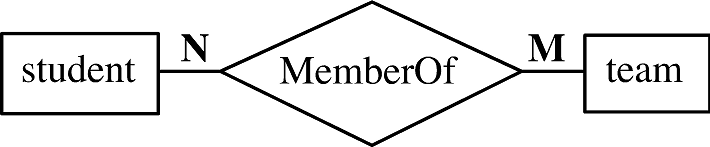
\includegraphics[scale=0.4]{../figures/chapter2/ER_example.png}
	\caption{ER diagram minimal example}
	\label{fig:ER_example}
\end{figure}

\begin{description}
\item[1) Entity type]\hfill \\
The most important artifact of ER is the entity.
It represents an individual and unambiguously identifiable object.
An entity is characterized by its properties.
An entity type is a template for entities that summarizes all attributes.
Entities can be seens as instances of an entity type with concrete values.
Graphically an entity type is a simple rectangle with its name in its center.

\item[2) Relationships]\hfill \\
Relationships can connect two or more entities and describe how they are interrelated.
In contrast to UML (see \ref{UML}) relationships are not simple lines, but are drawn as rhombus with the relationship name in its center.
This rhombus is then connected to two or more entities with simple lines.

\item[3) Attributes]\hfill \\
Attributes are properties of entites or relationship.
Graphically an attribute is a single ellipse with its name in its center.
It is connected to an entity or to a relationship object with the help of a simple line.
\end{description}


%cardinality: 1 C N NC
%The data modeling technique can be used to describe any ontology (i.e. an overview and classifications of used terms and their relationships) for a certain area of interest

%chen, kähenfuß, pfeilnotation, numeric, bachman

%recursive

%similar to clas diagram --> compact form (EWI)

\subsection{RBAC notation by Sandhu}
\label{RBAC_notation}
%Sandhu useda notation to visualize his proposal to roled-based access control
%maybe my own gsl from bachelor thesis?



\section{Gestalt laws and human optical perception}
\label{gestalt_laws_and_human_optical_perception}


\subsection{Gestalt laws}
\label{gestalt_laws}


\subsection{Human optical perception}
\label{human_optical_perception}




\section{GUI Design}
\label{gui_design}


\subsection{Design Patterns}
\label{design_patterns}


\subsection{Usability}
\label{usability}




\cleardoublepage
\chapter{Design: Graphical specification language}
\label{gsl_design}


\section{Concept}
\label{gsl_concept}
approach, basic ideas, adoptions from literature

\section{Elements}
\label{gsl_elements}


\section{Relationships}
\label{gsl_relationships}


\section{Structure}
\label{gsl_structure}


\section{Visualization on the higher abstraction level}
\label{higher_abstraction_level}




\cleardoublepage
\chapter{Design: Editor GUI}
\label{editor_design}


\section{Structure}
\label{editor_structure}


\section{Sections}
\label{editor_sections}




\cleardoublepage
\chapter{Implementation}
\label{implementation}
	
	
\section{Implementation base}
\label{implementation_base}
Qt, MVC

\section{Structure}
\label{implementation_structure}
	
	
\section{GUI sections}
\label{implementation_sections}




\cleardoublepage
\chapter{Evaluation}
\label{evaluation}


\section{Graphical specification language}
\label{evaluation_gsl}


\section{Editor}
\label{evaluation_editor}


\cleardoublepage
\chapter{Conclusion}
\label{conclusion}
\blindtext



\cleardoublepage
\chapter{Summary}
\label{summary}
\blindtext



% Anhang
%\cleardoublepage
%\tocentry{Anhang}
%\renewcommand{\thesection}{\Alph{section}}
%\markboth{Anhang}{}
%\chapter*{Anhang}
%\section{Kapitel 1}
%\section{Kapitel 2}
%\label{appendix}




% Literaturverzeichnis
\cleardoublepage
\DeclareRobustCommand{\citeext}[1]{\citeauthor{#1}~\cite{#1}}
\bibliographystyle{plainnat}

\bibliography{other/db}

\tocentry{Bibliography}





\end{document}